\section{Implementation}\label{sec:Implementation}
% ! Nuclear option: Linux dual-boot and screenshot as you go on it.

\subsection{Software requirements}
% Talk about Visual Studio Code.
% Talk about Python and the modules themselves. Did any of them have logins?
% Talk about OpenAI setup.
The project was developed using Visual Studio Code as a development environment and Python as the programming language.
Both of these are available freely with no limitation for academic use.

\para Many Python modules were used, with the UV package manager \autocite{astralUv} being used for their installation 
due to its own high speed and ease of use. The version of Python used was 3.10.16 to ensure compatibility with the wide variety 
of modules used, which are detailed in Table \ref{tab:PythonModules}.

\begin{longtable}{ | p{0.25\textwidth} | p{0.7\textwidth} | }
    \hline
    \cellcolor{blue!25} Module(s) & \cellcolor{blue!25} Purpose \\
    \hline
    langchain & The framework used to handle LLM interactions, as well as embedding documents and user queries. \\
    \hline
    langchain-community & Provides additional helper classes and functions to assist development. \\
    \hline 
    langchain-openai \newline 
    openai & Provides the functions used to interact with OpenAI models such as gpt-4o-mini and text-embedding-3-small in LangChain. \\
    \hline 
    langgraph & Used to create a directed sequence of events for the chatbot to execute. A major part of the backend, further described 
    in Section \ref{sec:ChatbotBackend}. \\
    \hline
    pdfminer-six \newline 
    pypdf & Dependencies of LangChain for PDF reading. \\
    \hline 
    Streamlit & Used as the frontend of the chatbot and also stores the conversation in memory. Described further in Section 
    \ref{sec:ChatbotFrontend}. \\
    \hline
    \caption{The Python modules used in the project's development.}\label{tab:PythonModules}
\end{longtable}



\subsection{Data storage}
% Talk about getting University policies from their site. Provide URL or Harvard reference it?
% Talk about your own added info document you made in LaTeX.
% Talk about embedding the policies.
The backbone of this project is the BCU-related data that the chatbot will pull from when queried.
The vast majority of this data was sourced from the official Birmingham City University website \autocite{bcuPoliciesProcedures},
where individual policies are stored as PDF files for public download without any access limitations or restrictions.
An observation made through an analysis of many of the policies was that none of them explicitly state key information about the university,
such as campus building locations or information about its student union. Therefore, an additional document of my own creation with \LaTeX
was included amongst the downloaded data. This document contained key information about BCU itself, with information on campus addresses 
and miscellaneous helpful information for students.

\para With all documents downloaded or created, the next stage would be to incorporate them in a format an LLM can interpret. This introduces 
LangChain, a popular framework for LLM app development \autocite{langchain_introduction_nodate}, which provides helper classes to directly read 
PDF files from a directory and split the text data within into smaller chunks, as seen in Figure \ref{fig:LangChainDocumentLoader}.

\begin{figure}[H]
    \centering
    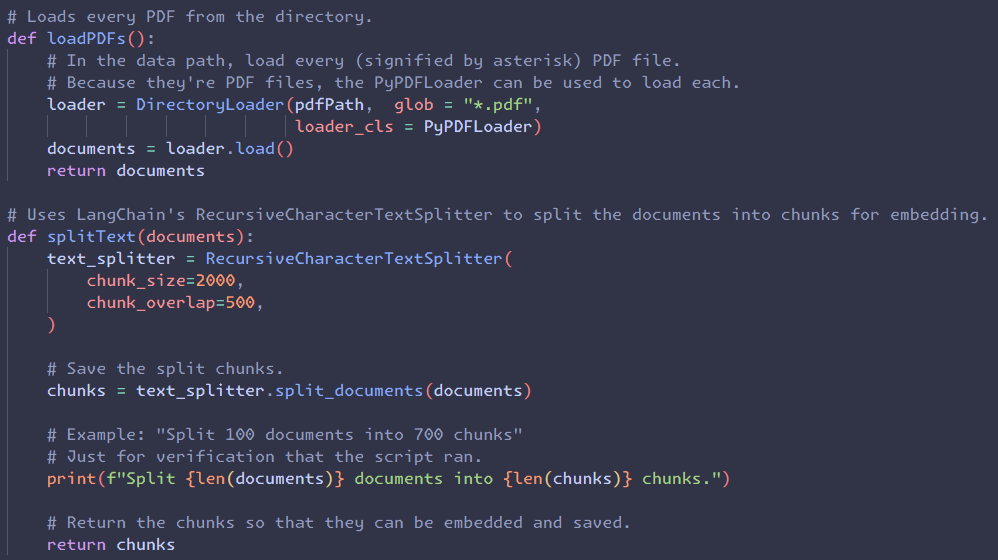
\includegraphics[width=0.8\textwidth]{Artefact/DocumentLoader.png}
    \caption{Code used to load all PDFs from the Policies directory and split them into chunks. \label{fig:LangChainDocumentLoader}}
\end{figure}

\noindent Multiple chunk sizes and overlaps were tested during the artefact's development, with an eventual settlement on 2000 character 
chunks with 500 character overlaps being used. Maximising the size of chunks is a key part in assisting the chatbot's retrieval process,
as it will be able to fetch more data with a single query which allows it to answer questions with greater detail and factual accuracy.
The chunk overlap defines how many characters appear across multiple sequential chunks, ensuring that key information is unlikely to be 
split over multiple chunks where the chatbot then may be unable to cite it. LangChain's RecursiveCharacterTextSplitter also provides 
additional arguments for a custom length function if desired, though there was no need in this project, as well as adding start indexes 
to each vector, which adds metadata stating the numerical ID of each chunk as determined by the sequential order they are split in. 

\para Once these chunks have been created, they must then be embedded as vectors, which will allow an LLM to interpret them. These 
vectors were then stored in a Facebook AI Similarity Search (FAISS) database as researched in Section \ref{sec:LitReviewRAG}, which 
ensured that the policies only needed to be embedded once rather than every time the chatbot was run, and would be retrieved 
at high speeds thanks to FAISS' efficiency.

\begin{figure}[H]
    \centering
    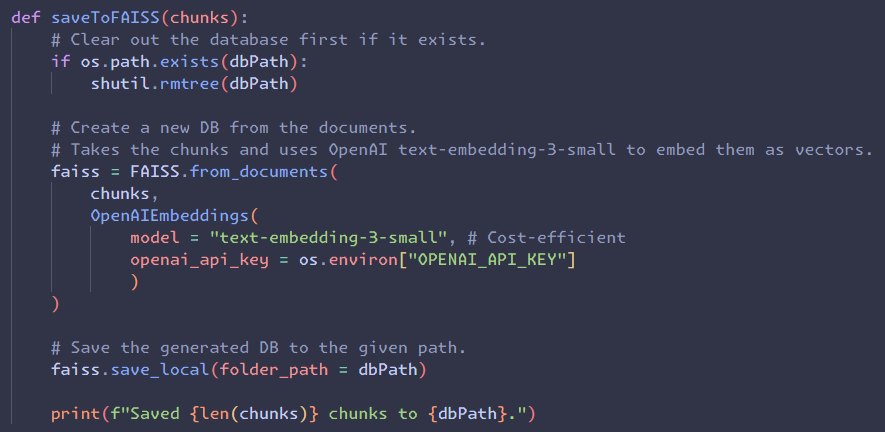
\includegraphics[width=0.8\textwidth]{Artefact/SaveToFAISS.png}
    \caption{Code used to embed and store the chunks into a FAISS DB. \label{fig:LangChainStoreFAISS}}
\end{figure}

\noindent Firstly, any existing database in the specified directory is cleared to ensure that there are no I/O errors when attempting 
to save to the directory. LangChain provides wrapper functions for both the embedding and storage of this data, making it a smooth 
and simple process in very few lines of code. 

\para The embedding model used is OpenAI's text-embedding-3-small model \autocite{openai_vector_nodate}. The motivation behind the use of this model 
was primarily due to its cost efficiency, with OpenAI approximating 62,500 pages can be embedded for each dollar spent. For each 
2000-character chunk, the embedding model translates it into vector space for the LLM's interpretation. The vectors are produced based on the 
semantic similarities of each word as previously discussed and visualised in Section \ref{sec:LitReviewNLP}. 

\begin{figure}[H]
    \centering
    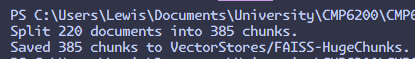
\includegraphics[width=0.8\textwidth]{Artefact/EmbeddingConsoleSmall.png}
    \caption{The PDF to vector store conversion code successfully running. \label{fig:EmbeddingConsole}}
\end{figure}



\subsection{Backend code}\label{sec:ChatbotBackend}
% Talk about LangChain and LangGraph.
As previously mentioned, the core functionality of the chatbot was developed using the LangChain and LangGraph frameworks. LangChain in particular
simplifies the development process by providing various functions and classes for quick and easy integration with necessary services such 
as FAISS and the OpenAI API, with LangGraph defining the chatbot's structure as depicted in Figure \ref{fig:ChatbotLangGraph}. 

\begin{figure}[H]
    \centering
    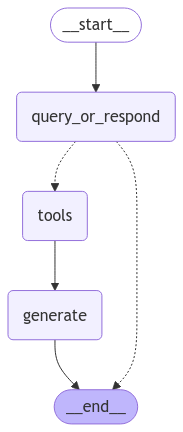
\includegraphics[width=0.3\textwidth]{Artefact/LangGraph.png}
    \caption{The graph for the chatbot. \label{fig:ChatbotLangGraph}}
\end{figure}


\para Before detailing each node of the graph, it is first necessary to establish some prerequisite variables such as the LLM itself. 
The LLM used is OpenAI's gpt-4o-mini due to cost-efficiency. The difference in performance between 4o-mini and 4o was deemed not significant 
enough for the price increase of 1500\% per 1 million tokens in relation to 4o-mini \autocite{openaiPricing}, especially considering that 4o-mini
performs suitably for the task at hand.

\para Figure \ref{fig:PrelimVariables} shows each of the variables being established, including the LLM, 
via LangChain's 'init\_chat\_model' function. The LLM is initialised with a temperature of 0, which means that it should give the same 
answer to the same prompt whenever it is given. As mentioned, this does reduce the 'personality' of the chatbot, though it greatly helps 
to reduce the potential for hallucinations in a Q\&A RAG scenario such as this one.

\begin{figure}[H]
    \centering
    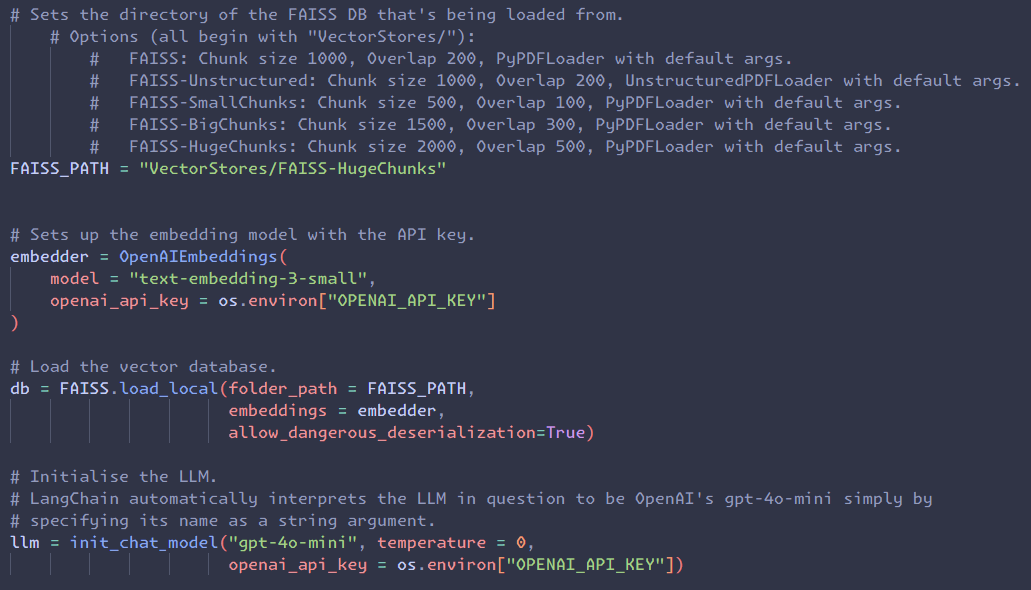
\includegraphics[width=\textwidth]{Artefact/PrelimVariables.png}
    \caption{Establishing prerequisite variables for the chatbot. \label{fig:PrelimVariables}}
\end{figure}

\noindent Thorough experimentation with the chunk sizes previously discussed in Figure \ref{fig:LangChainDocumentLoader} occurred during 
development, with the eventual decision of settling on the 2000-character chunks being made due to its more reliable performance on a set 
of sample questions discussed in Chapter \ref{ch:Evaluation}. Following the relative directory of the FAISS database being set, the 
OpenAI embedding model is once again used so that similarity searches may be performed on the database. An additional argument,
'allow\_dangerous\_deserialization', is given when loading the database. When a FAISS database is saved using LangChain, it is saved as a 
serialized file known as a Pickle file, using a .pkl file extension. It is possible for malicious code to be embedded inside these files
which could be executed when they are deserialized. However, as the files were generated specifically for this project and their contents 
are already known, it is safe to deserialize them.

\para With the prerequisite variables established, the first node of the graph was created. This is the core functionality of the LangGraph 
module, which builds on LangChain by defining an app's workflow 
as nodes and edges on a graph \autocite{langgraphLangGraph}. In development, these nodes and edges can be created, with support for conditional 
edges that ensure certain nodes such as tool calls only activate when necessary. This allows for the creation of self-directed agents which make 
decisions independently, with this functionality being used in the chatbot to decide whether a response needs BCU-related context or not. This 
occurs in the first node and entry point of the graph: the 'query\_or\_respond' node.

\begin{figure}[H]
    \centering
    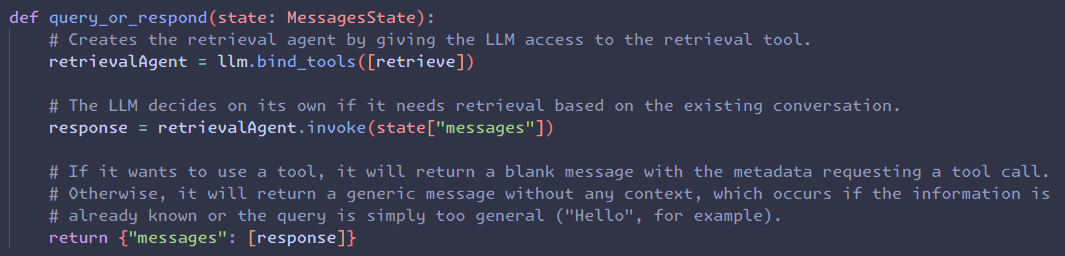
\includegraphics[width=\textwidth]{Artefact/QueryOrRespond.png}
    \caption{Code used for the 'query\_or\_respond' graph node. \label{fig:QueryOrRespond}}
\end{figure}

\noindent This function clearly demonstrates LangChain's abstractions of the backend functionality; these three lines of code
serve as the entire decision-making logic for this node, as the LLM itself will decide whether it can immediately answer the user's query,
such as in a scenario where the information they are requesting is already known from earlier in the conversation, or if their query is too 
general such as stating their name. If the LLM decides it cannot answer the query with the information it currently has available within 
the conversation, it will instead invoke the left conditional branch of the graph in Figure \ref{fig:ChatbotLangGraph} by calling on the 
retriever tool denoted in Figure \ref{fig:RetrieverTool}.

\begin{figure}[H]
    \centering
    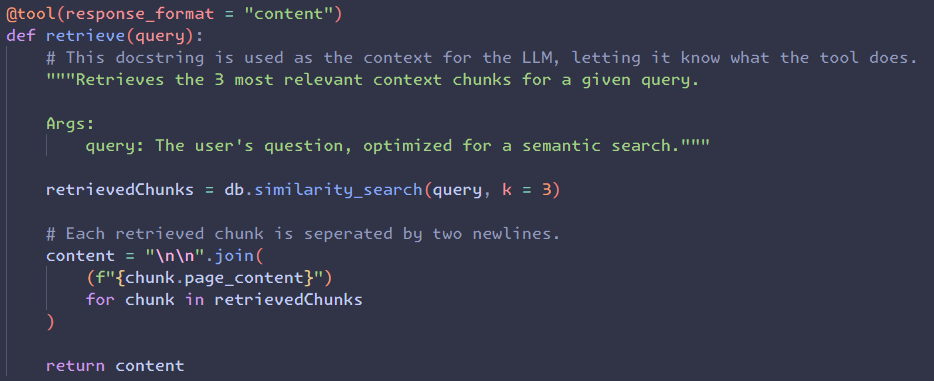
\includegraphics[width=\textwidth]{Artefact/Retriever.png}
    \caption{Code used for the retrieval tool. \label{fig:RetrieverTool}}
\end{figure}

\noindent Using the '@tool' decorator informs LangChain that the following function is a tool to be used by the LLM.
% The tool's response format is set to content, meaning that it will return the results as a LangChain 'ToolMessage', 
% which is beneficial for the frontend as these can be manually hidden from the user. 
The retriever tool itself is simplistic 
in function: it will perform a semantic search on the FAISS database based on the user's query. LangChain enforces that all 
tools require a Python docstring explaining their function, as the LLM will read this docstring to understand what the tool 
is and how to use it. By specifying that the 'query' argument should be optimised for a semantic search, the 'query\_or\_respond'
node will output a modified version of the user's query as the input to the tool, which is further discussed in Section 
\ref{sec:ChatbotFrontend}. 
% ! Show this happening? 

\para When the 3 most similar chunks have been retrieved as defined by 'k' in the similarity search method, the text of each chunk 
is saved and separated by two newline characters to assist the LLM in understanding they are not part of the same text. The large 
text block is then returned as this tool's output, ready to then be passed into the 'generate' node. 

\begin{figure}[H]
    \centering
    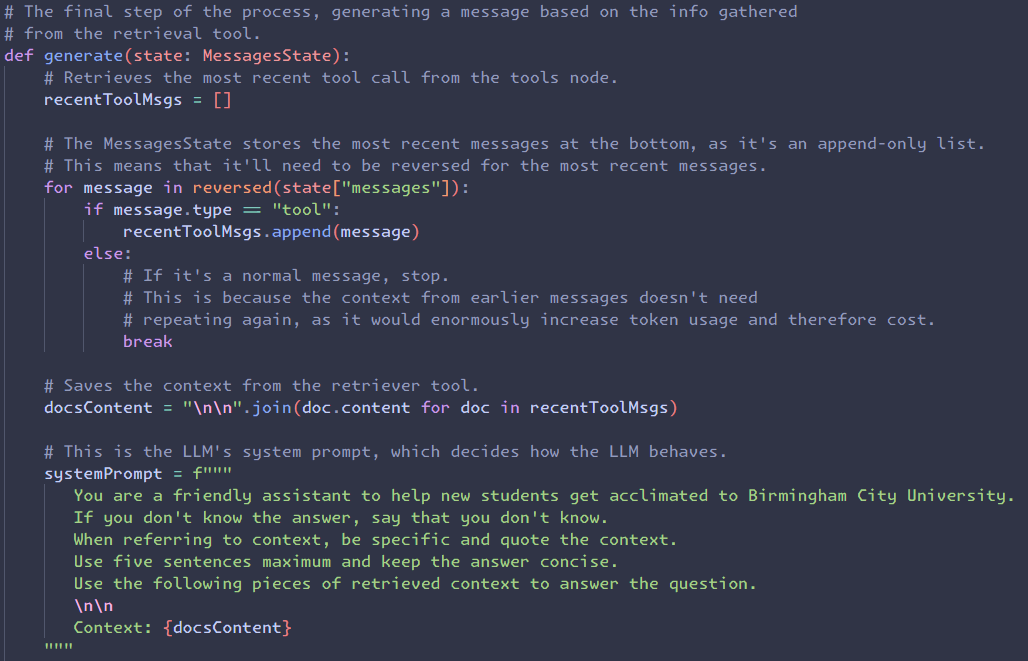
\includegraphics[width=\textwidth]{Artefact/Generate1.png}
    \caption{Code used for the 'generate' node (1/2). \label{fig:Generate1}}
\end{figure}

\noindent The 'generate' function is the largest function of the chatbot, and is split across 
Figures \ref{fig:Generate1} and \ref{fig:Generate2}. In the interests of saving 
cost, time and the potential risk of maximising the LLM's context window, the most recent retrieval tool 
call is saved. This tool call contains the RAG context from the retrieval tool, and will be at least 
6,000 characters in length due to the previously mentioned chunk sizes and amount of chunks retrieved.
This most recent tool call is the only context given to the LLM to reduce the token cost of each prompt 
and to mitigate any potential confusion if the LLM is given thousands of words of input context.

\para The retrieval tool returns three LangChain Document objects, each containing one chunk.  
Therefore, the content of each of these Documents is extracted and saved before being appended to the 
LLM's system prompt.

\para The system prompt is a massive part of LLM usage, and almost entirely dictates what the LLM will do 
based on any given input. The prompt is written in natural language which is interpreted by the LLM as a set 
of instructions to follow at all times. As such, the prompt given for the chatbot defines that it is 
a BCU assistant which should specifically quote context and keep all answers brief (for cost efficiency).
This prompt was found to be highly effective, with the LLM responding with mostly satisfactory results as 
detailed in Chapter \ref{ch:Evaluation}.

\begin{figure}[H]
    \centering
    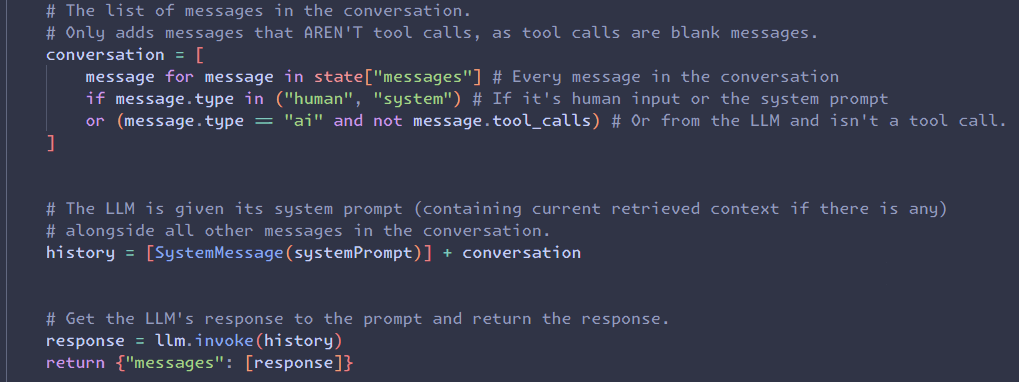
\includegraphics[width=\textwidth]{Artefact/Generate2.png}
    \caption{Code used for the 'generate' node (2/2). \label{fig:Generate2}}
\end{figure}

\noindent With the system prompt prepared, the LLM should also account for the current conversational 
history, which is retrieved from the LangGraph MessagesState. The MessagesState is an append-only list 
containing all messages in the current conversation, stored as a HumanMessage, AIMessage, or SystemMessage.
These are three LangChain objects used to represent the various actors in a conversation: the human user,
the LLM and the system prompt.

\para When retrieving the current conversation, tool calls are excluded. This is because through experimentation,
it was discovered that when the chatbot calls on a tool, it generates a blank message with metadata indicating a
tool call. This blank message is not relevant, and therefore does not need to be included in the conversational history.

\para Finally, the new system prompt is inserted as the most recent message in the conversation, and the LLM
is invoked with the filtered conversation history, with the generated response being returned.

\begin{figure}[H]
    \centering
    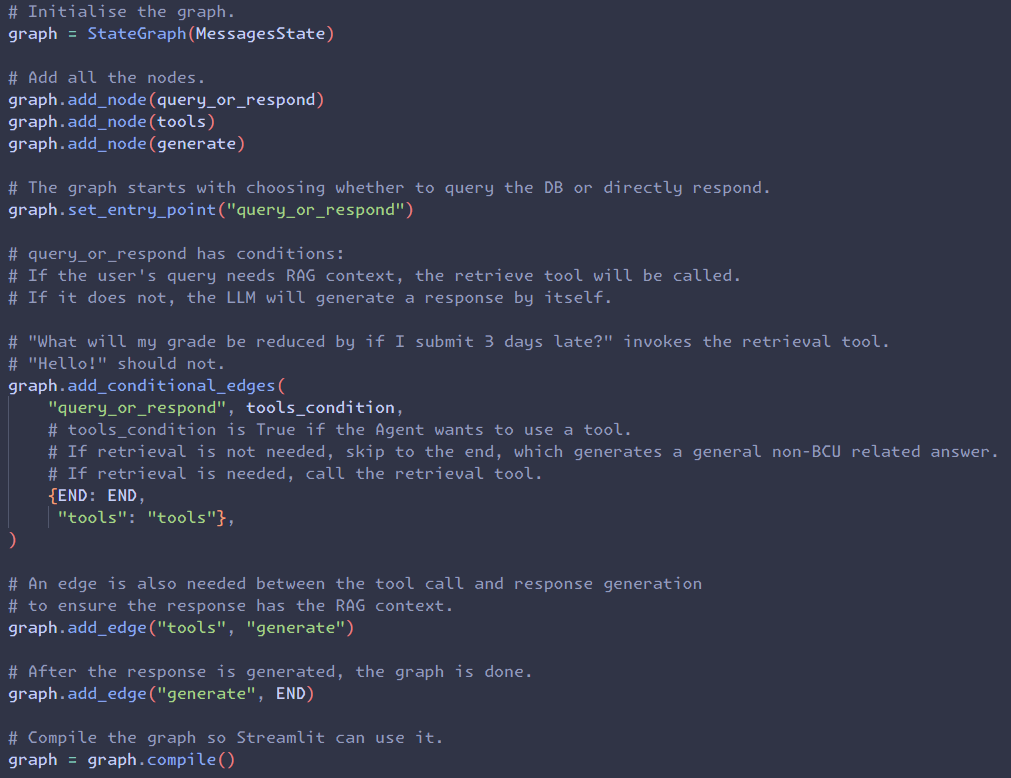
\includegraphics[width=\textwidth]{Artefact/LangGraphCode.png}
    \caption{Code used to form the graph. \label{fig:LangGraphCode}}
\end{figure}

\para To conclude the chatbot's backend Python script, the LangGraph is created using the conditions mentioned 
previously. A particularly helpful feature of LangGraph for this scenario was 'tools\_condition', which is
set to True if the LLM calls on a tool, and False if it does not. Based on this condition, the graph will either 
go down the left branch, invoking the retrieval tool and generating a contextualised response, or it will skip 
directly to the end, where the LLM will generate a generic answer without any RAG.


\newpage 

\subsection{Frontend code}\label{sec:ChatbotFrontend}
% Talk about Streamlit.
% Show example conversations here or perhaps make another section for them.
The chatbot's frontend GUI was created using the Streamlit package, which allows for the creation of visually appealing, dynamic and 
responsive web apps through simple Python code \autocite{streamlitStreamlitFasterWay2021}. Figure \ref{fig:StreamlitInitPage} shows 
the initial variables set for the page's structure.

\begin{figure}[H]
    \centering
    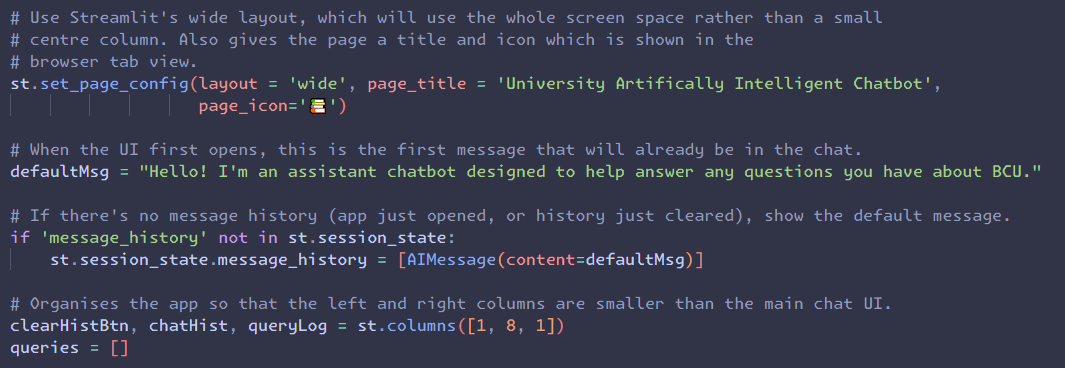
\includegraphics[width=\textwidth]{Artefact/Streamlit/Backend/PageInit.png}
    \caption{The variables defining the frontend page's structure. \label{fig:StreamlitInitPage}}
\end{figure}

\noindent Streamlit provides many helpful methods and variables for creating the frontend GUI, allowing for the page layout to be 
quickly defined using 'set\_page\_config', where the wide layout was used to ensure the app fills the screen, and the title and an icon 
for the browser tab are also provided. 

\para When the app initially opens, it would by default open to a mostly blank page. To remedy this, a default message was provided 
explaining what the chatbot is, which will always show as the first message in the conversation. This is performed by validating that 
the current session's message history is empty before inserting the default message.

\para Following this, three columns are set up on the page: a small column containing a button to clear the current message history,
a large column containing the main chat UI, and another small column showcasing the queries being given to the FAISS database by the 
chatbot, which would be none at the time of startup, so an empty list is defined.

\para After the page's structure is defined, the functionality of each of the three columns is established as depicted in Figures \ref{fig:StreamlitLRColumns}, \ref{fig:StreamlitMainColumn1} and \ref{fig:StreamlitMainColumn2}.

\begin{figure}[H]
    \centering
    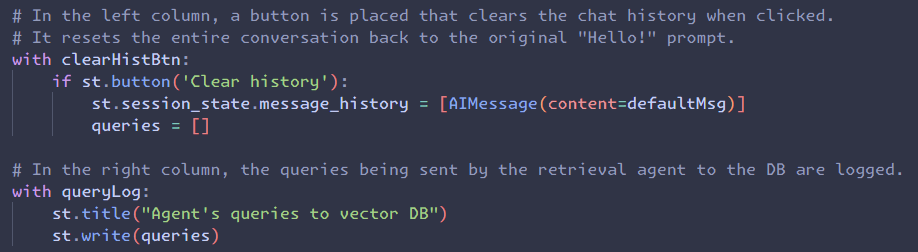
\includegraphics[width=\textwidth]{Artefact/Streamlit/Backend/LRColumns.png}
    \caption{Defining the left and right column functions. \label{fig:StreamlitLRColumns}}
\end{figure}

\noindent The left column ('clearHistBtn') has a button placed in it which will clear the current conversational history when clicked,
and also empty the list of queries to the database. This button effectively resets the app to its initial opening state.

\para The right column ('queryLog') outputs all the agent's queries which it has given to the vector database. The queries themselves are 
retrieved within the main column of the app, 'chatHist'.

\begin{figure}[H]
    \centering
    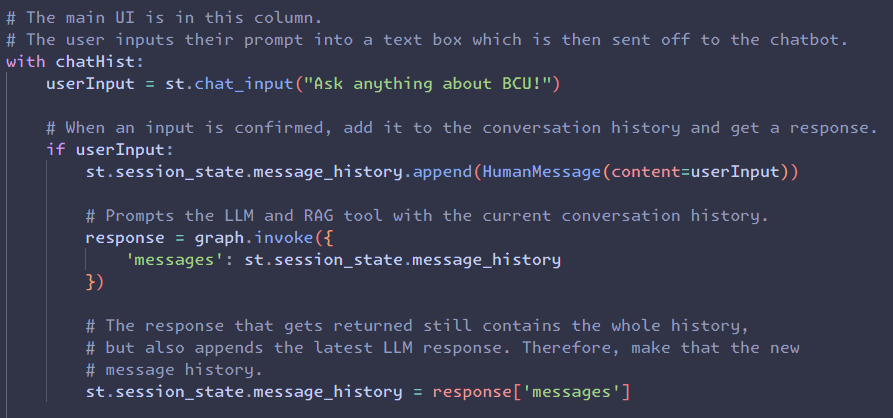
\includegraphics[width=\textwidth]{Artefact/Streamlit/Backend/MainColumn1.png}
    \caption{Defining the main column function (1/2). \label{fig:StreamlitMainColumn1}}
\end{figure}

\noindent The user's input box is established, and when an input is given, it is added to Streamlit's active 
conversation history, which is then used to invoke the chatbot's LangGraph. When the chatbot responds, it returns 
the entire conversation history once again, this time containing the chatbot's latest response. Therefore, this is used 
to overwrite the existing Streamlit history.

\para With the core prompting functionality set, the Streamlit UI for this column then needed to be established as depicted 
in Figure \ref{fig:StreamlitMainColumn2}.

\begin{figure}[H]
    \centering
    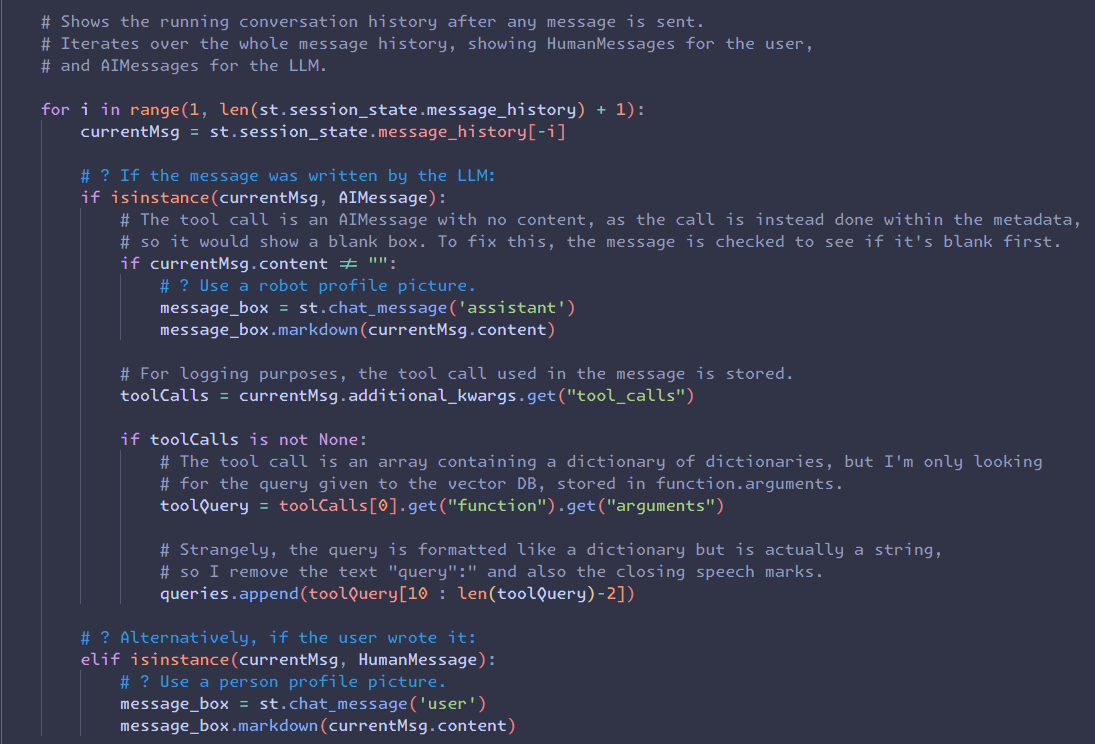
\includegraphics[width=\textwidth]{Artefact/Streamlit/Backend/MainColumn2.png}
    \caption{Defining the main column function (2/2). \label{fig:StreamlitMainColumn2}}
\end{figure}

\noindent By iterating over each message in the conversation, logic is established to determine whether the message should 
use a human profile picture or a robot profile picture, representing the user and chatbot respectively. Initially, a bug was 
present where the chatbot would send two messages at a time, with one message being blank. It was previously established that 
this was due to the 'query\_or\_respond' node invoking the retrieval tool, which it does in the form of a blank message with 
metadata. However, Streamlit would still detect this blank message and output it. Therefore, the chatbot's message is checked 
to ensure it is not blank before being displayed. If it is blank (i.e. a tool call), it will not be displayed to the user, as 
there would be no reason for this, and it would only serve to cause confusion.

\para Logging the tool calls for the 'queryLog' column proved to be somewhat challenging. The metadata of an AIMessage ('additional\_kwargs')
is structured like a dictionary, though cannot entirely be parsed in the same way. Therefore, after parsing as far as possible using the 
standard dictionary 'get' method, extracting the actual query itself is performed with basic string manipulation, to exclude irrelevant 
details from the query string. This sanitised string is then logged as a query which will be automatically detected by the 'queryLog' column
and output.

\newpage 

\subsection{Running the chatbot}\label{sec:ChatbotRun}
After ensuring all prerequisite packages are installed, the chatbot itself is run through the 'Streamlit Frontend' file. Because the file 
is executed by Streamlit rather than the generic Python interpreter, it is run slightly differently as depicted in Figure \ref{fig:RunApp}.

\begin{figure}[H]
    \centering
    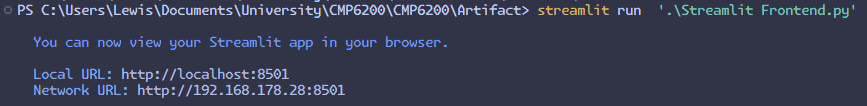
\includegraphics[width=\textwidth]{Artefact/Streamlit/Frontend/CMD.png}
    \caption{Running the chatbot from the terminal with Streamlit. \label{fig:RunApp}}
\end{figure}

\noindent Then, by navigating to the given URL, the chatbot itself can be accessed.

\begin{figure}[H]
    \centering
    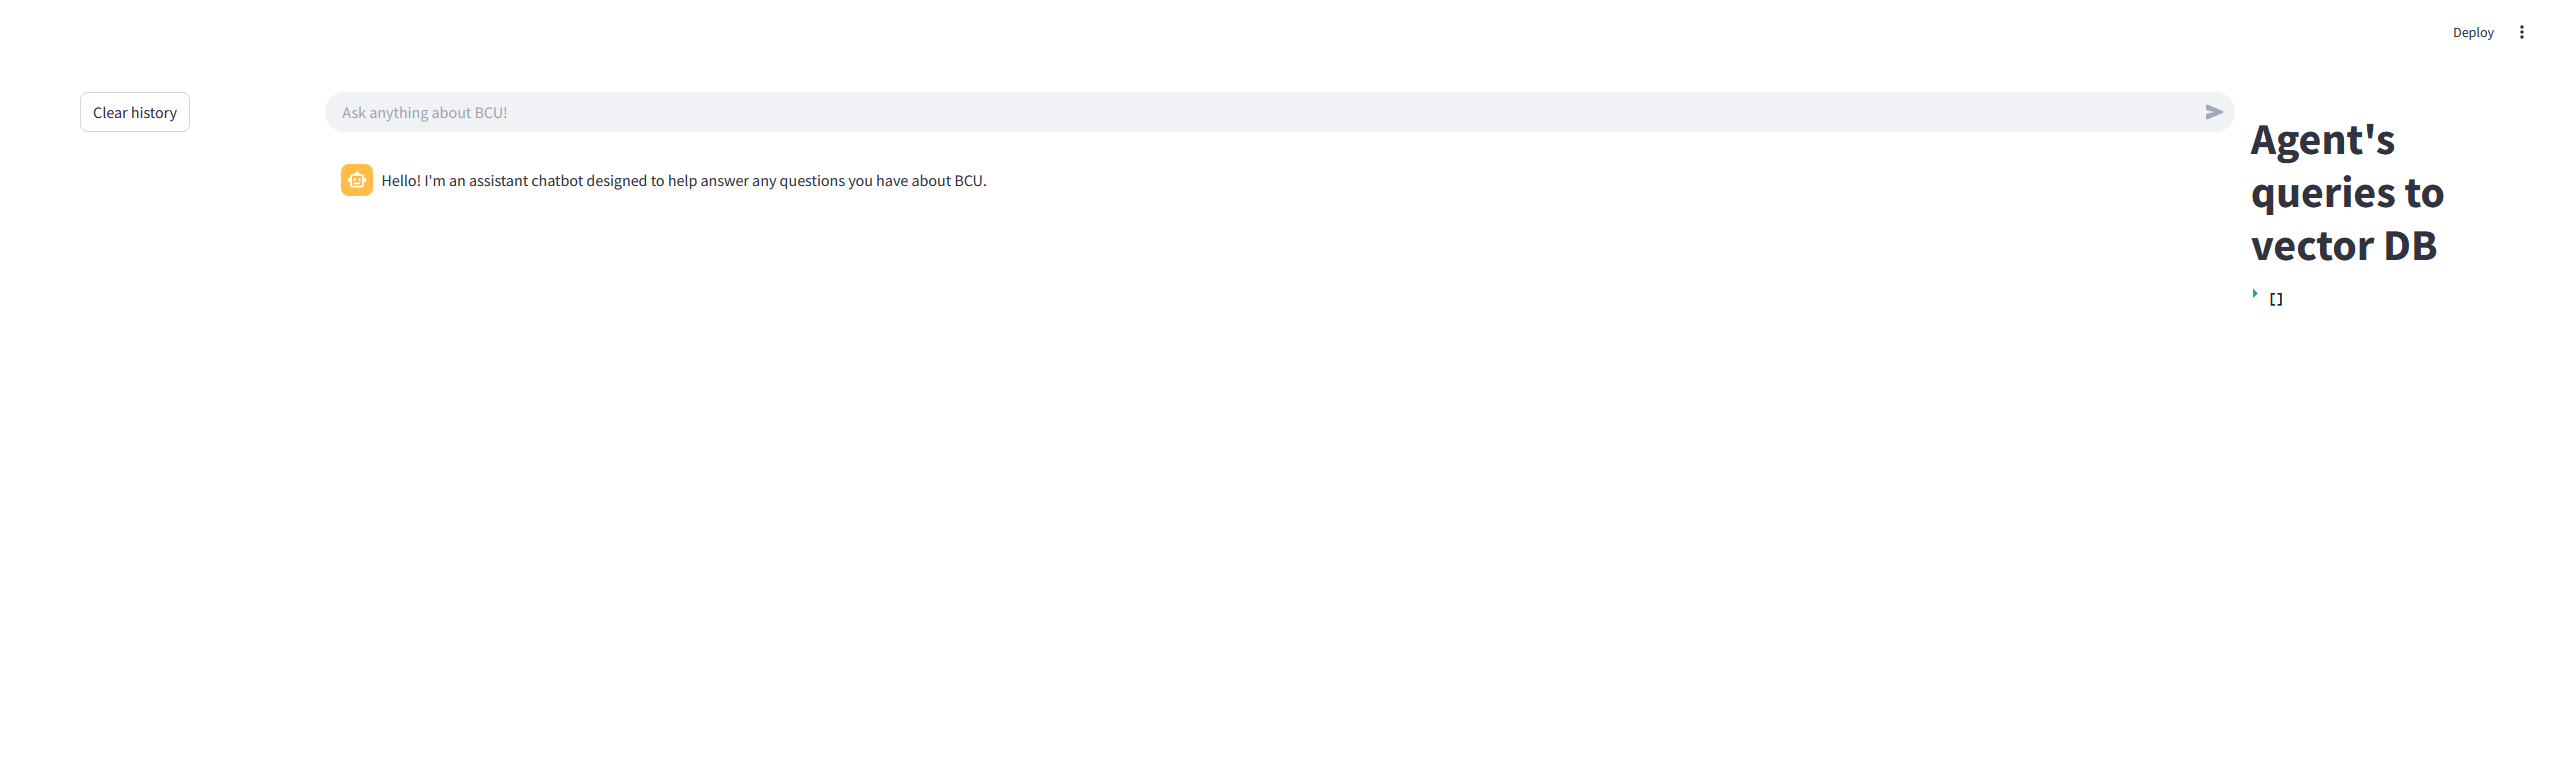
\includegraphics[width=\textwidth]{Artefact/Streamlit/Frontend/FirstRun.png}
    \caption{The chatbot's GUI at its initial state. \label{fig:FirstRun}}
\end{figure}

\noindent The previously defined columns are clearly visible: 'clearHistBtn' as the 'Clear history' button on the left, 'chatHist' as the main 
central column with the text box and default chatbot message, and 'queryLog', currently showing the empty list of queries. 

\para The chatbot can now be queried by simply giving a prompt in the main text entry field as shown in Figure \ref{fig:FirstQuery}, 
which is slightly zoomed in for demonstrative purposes.

\begin{figure}[H]
    \centering
    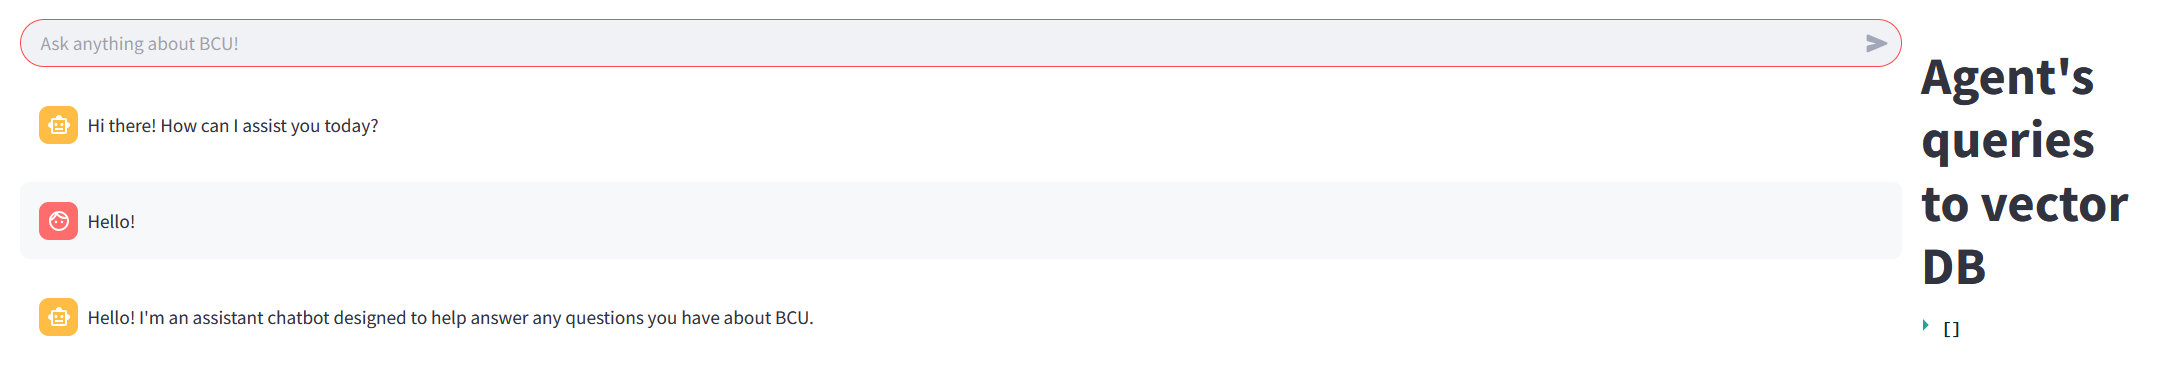
\includegraphics[width=\textwidth]{Artefact/Streamlit/Frontend/FirstQuery.png}
    \caption{Prompting the chatbot with 'Hello!'. \label{fig:FirstQuery}}
\end{figure}

\noindent This simple query demonstrates the conditional branch in LangGraph. With 'Hello' being such a simple query, the chatbot deems 
it unnecessary to retrieve context for, as it can already provide a suitable answer. This can be seen from the 'queryLog' column still 
remaining empty. Instead, the chatbot can now be asked a BCU-related question which it will require context for.

\begin{figure}[H]
    \centering
    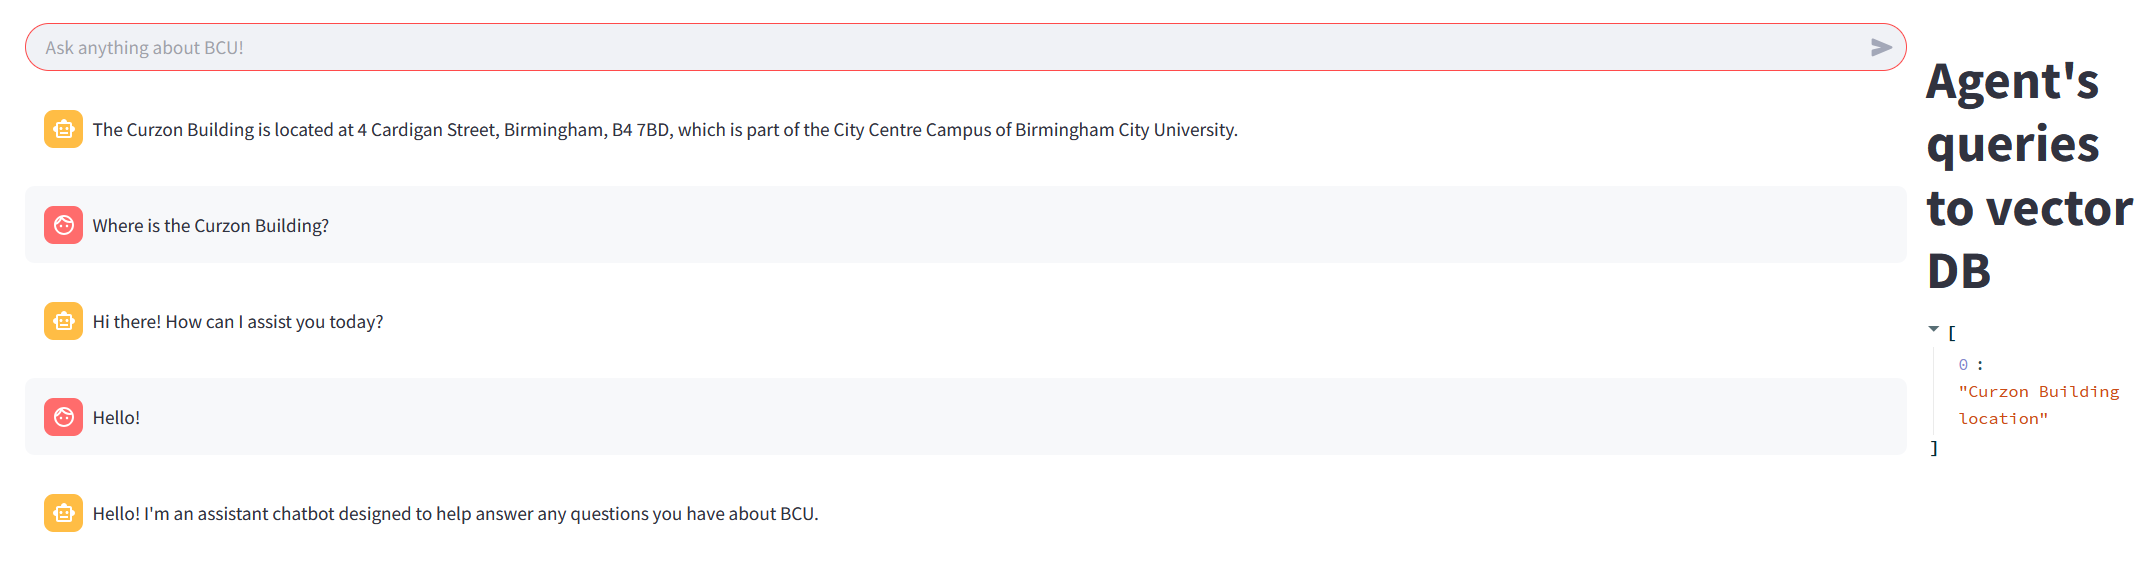
\includegraphics[width=\textwidth]{Artefact/Streamlit/Frontend/SecondQuery.png}
    \caption{Prompting the chatbot with 'Where is the Curzon Building?'. \label{fig:SecondQuery}}
\end{figure}

\noindent The chatbot is able to answer correctly with no hallucination, as it performed a search for 'Curzon Building location' on the 
FAISS database as shown in the 'queryLog' column. From this, it was able to parse the retrieved chunks, locate the address, and return it to the
user. To expand on this functionality, another relevant question can be asked:

\begin{figure}[H]
    \centering
    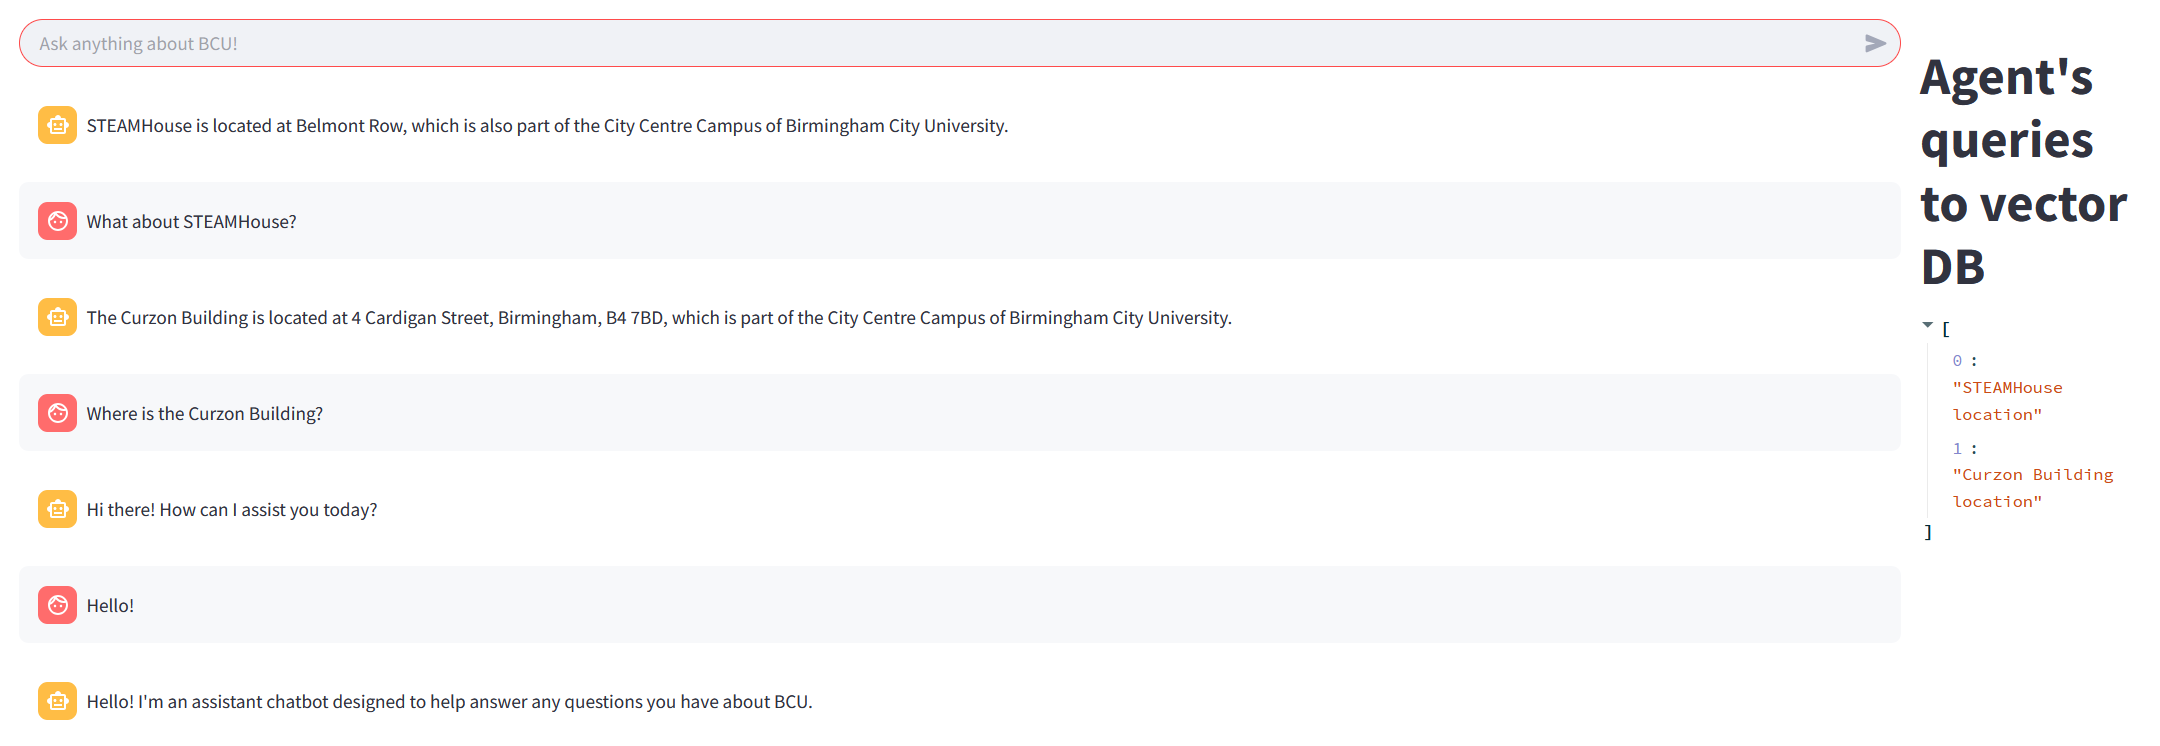
\includegraphics[width=\textwidth]{Artefact/Streamlit/Frontend/ThirdQuery.png}
    \caption{Prompting the chatbot with 'What about STEAMHouse?'. \label{fig:ThirdQuery}}
\end{figure}

\noindent Because the chatbot is invoked with the conversation history, it is able to interpret what the user means by 'What about', 
referring to another building's location. As such, it uses another similar query on the vector database, this time retrieving information 
for the STEAMHouse building, which it is able to successfully return to the user. Additionally, its response states 'which is also part of 
the City Centre Campus', showing that the previous response it gave was factored into its new response, as per the use of 'also'.

\begin{figure}[H]
    \centering
    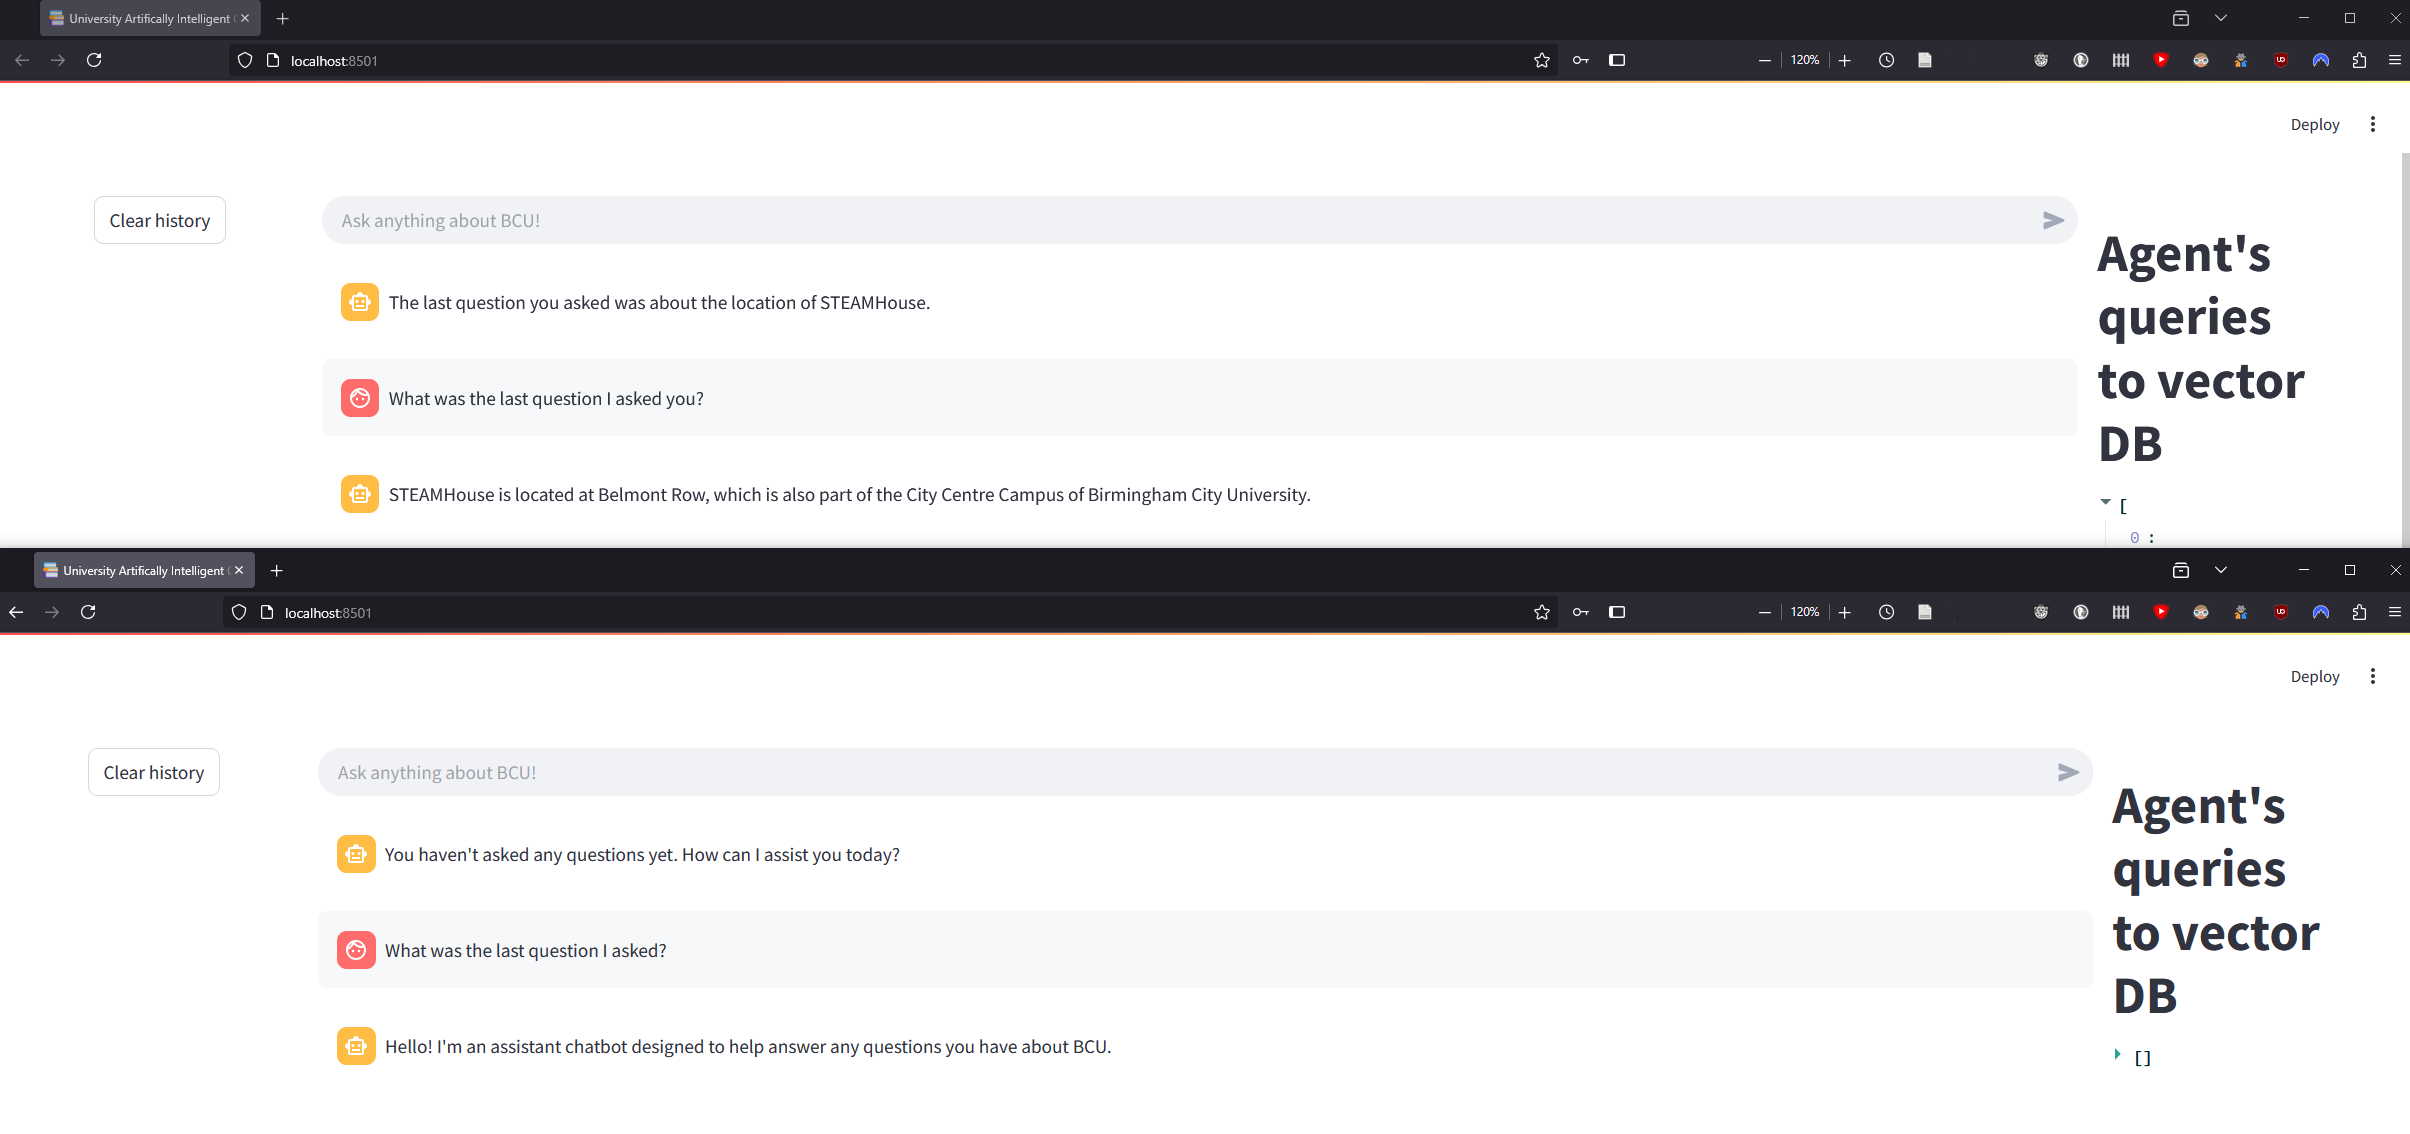
\includegraphics[width=\textwidth]{Artefact/Streamlit/Frontend/UniqueConversations.png}
    \caption{Two separate chatbot instances, which run without memory overlap. \label{fig:UniqueConversations}}
\end{figure}

\noindent Figure \ref{fig:UniqueConversations} depicts how multiple instances of the chatbot can run at the same time without influencing 
each other, which is a key element in terms of user privacy. In the figure, it can be seen that two separate windows of the chatbot are 
running, where one contains the conversation in Figure \ref{fig:ThirdQuery} and another that had just been started. Both chatbots are 
asked what the last question asked of them was, which the new instance cannot answer, but the old instance can. This shows how the second 
chatbot instance runs independently of the first.

% ! What more can really be said?